\part{Agentivité et langage}

\chapter{Une définition de l’agentivité}
%wrong title 

\section{\textit{The Big Two} : Agentivité et Communion}

Parmi toute la littérature psychologique qui cherche à définir la structure de la personnalité humaine, le modèle des \textit{Big Five} est souvent retenu. Comme son nom l'indique, il s'agit d'un modèle descriptif de la personnalité fondé sur cinq traits centraux (Neuroticisme, Extraversion, Ouverture, Agréabilité et Conscienciosité). Construits par analyse factorielle, ces traits représentent les intercorrélations de comportements spécifiques et répétés, et sont largement supposés constituer les dimensions indépendantes les plus élevées dans la structure hiérarchique de notre personnalité. En d'autres termes, la personnalité d’un individu, entendue ici comme un ensemble de traits comportementaux émis au sein de classes spécifiques définies par leur contenu dans un éventail de situations, et de manière cohérente dans le temps, serait tout au plus réductible à la combinaison de ces cinq traits fondamentaux.

Toutefois, il est apparu récemment que ces facteurs n'étaient pas totalement indépendants, à savoir qu'il existait toujours des corrélations entre certains d’entre eux\footnote{\cite{block_contrarian_1995}}\footnote{\cite{egan_neo-ffi_2000}}. De là ont été définies deux dimensions plus larges encore, qui constitueraient les strates les plus génériques au moment de décrire la structure de notre personnalité, et pour l'instant considérées comme véritablement orthogonales : l’Agentivité et la Communion, communément désignées par le modèle des \textit{Big Two}\footnote{Ces dimensions sont plus ou moins équivalentes aux facteurs Alpha et Beta proposés par {\cite{digman_higher-order_1997}}, et synthétisés chez Wiggins par les métaconcepts d'Agentivité et de Communion (\cite{wiggins_agency_1991})}.

Du latin \textit{agens}, qui signifie « agir » ou « faire quelque chose », l’agentivité est en réalité un concept aux multiples facettes, qui peut revêtir plusieurs significations plus ou moins intriquées. 

Tout d'abord, l’agentivité renvoie à « l'expérience du contrôle de ses propres actions et, à travers elles, des événements du monde extérieur ». C’est ce qu'on appelle plus précisément le « sentiment d’agentivité »\footnote{\cite{haggard_p_chambon_v_sense_nodate}}. En ce sens, l’agentivité est très proche du concept de « locus de contrôle », qui correspond à la croyance qu’un individu entretient sur la relation entre les actions qu’il entreprend et leurs résultats. Cette croyance peut être externe : la personne croit que des facteurs indépendants de sa volonté sont plus importants que ses propres actions au moment de façonner leurs résultats, ou bien interne : il se pense principal maitre à l’œuvre, ce qui correspondrait à un plus grand sentiment d’agentivité.

En relation avec le modèle des \textit{Big Two} cité plus haut, l’agentivité correspond également à « l'une des deux modalités fondamentales de l'existence humaine qui se manifeste dans le contenu de notre perception de nous-mêmes et des autres, dans notre comportement social et dans la manière dont notre personnalité fonctionne »\footnote{\cite{bakan_duality_1966}}. Contrairement à la communion, qui vise à se rapprocher des autres, l’agentivité est centrée sur la poursuite et la réalisation d'objectifs personnels. En ce sens, l’agentivité et la communion peuvent être considérées comme des aspects complémentaires de l'adaptation humaine, qui peuvent interagir pour façonner le comportement social\footnote{\cite{locke_agency_2014}}\footnote{\cite{wiggins_agency_1991}}. Ils répondent en effet à deux besoins fondamentaux en société : le besoin de s'assurer une position sociale avantageuse (ou l’affirmation de soi, étroitement liée à l’agentivité), mais qui doit être modulé avec le besoin d'être intégré dans le groupe (la coopération, soutenue par cette autre dimension psychologique qu’est la communion).

Enfin, l’agentivité peut être comprise comme une relation spécifique entre l'individu et son environnement social, impliquant à la fois un sentiment d’agentivité et une activité réelle, qui se manifeste par la réalisation d'un objectif.

S'appuyant sur cette nature protéiforme qu’il cherche à théoriser, Seligman\footnote{\cite{seligman_m_maymin_p_agency_2022}} considère que l’agentivité est synthétiquement composée de trois éléments : l'efficacité (l'état d'esprit selon lequel on peut atteindre un objectif spécifique maintenant), l'optimisme (l'état d'esprit selon lequel on peut atteindre cet objectif dans un avenir lointain) et l'imagination (l'état d'esprit selon lequel on peut atteindre de nombreux objectifs).

Hitlin et Edler\footnote{\cite{hitlin_time_2007}} ont également proposé une typologie intéressante de l'agentivité, plus directement fondée sur les horizons temporels des acteurs dans les situations d'action, et ses implications pour le soi, comme le détaille le tableau ci-après. Ce modèle nous servira d’heuristique connexe au moment de joindre les approches théoriques de l’agentivité et la psychologie sociale: 

\begin{figure}[!ht]
    \centering
    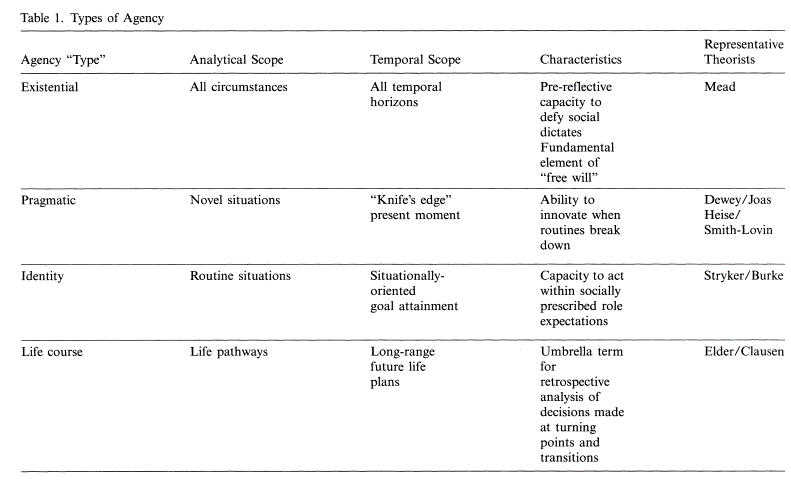
\includegraphics[width=16cm]{img/Types of agency.png}
    \caption{Typologie de l'agentivité s'appuyant sur l'horizon temporel de l'action - Hitlin et Edler (2007)}
    \label{Types_of_agency}
\end{figure}

Ainsi, sous quelque angle que ce soit, l’agentivité implique une activité volontaire et une concentration sur les objectifs de l'individu, qui va de pair avec l’élargissement de son horizon temporel ; et peut être considérée comme une différence individuelle. Plus finement encore, Vallacher\footnote{\cite{vallacher_levels_1989}} intègre la dimension d’agentivité dans sa « théorie de l'identification de l'action », pour en donner une définition qui servira d'inspiration à l'ensemble de ce projet de recherche. Selon lui, étant donné qu'un acte peut être identifié de nombreuses façons par l’individu qui l’exécute, les dispositions comportementales seront inévitablement insuffisantes pour représenter les régularités du comportement, ce qui remet en question la validité même de toute tentative globale de classification des comportements dans des catégories de traits de personnalité \textit{a priori}. Un schéma d'organisation plus raisonnable serait donné par la structure cognitive individuelle des identifications de l’action.

\section{La théorie de l’identification de l’action, ou l’existence d’un continuum agentif}

Pour Vallacher\footnote{\cite{vallacher_levels_1989}}, le niveau d’agentivité personnelle est défini comme « une dimension indépendante qui permet de distinguer à quel point un individu a organisé ses actions en catégories abstraites et significatives qui peuvent servir à canaliser le comportement en tendances dispositionnelles ». En bref, chaque individu pourrait être placé sur un continuum agentif, mesurant son niveau d'identification des actions qu'il entreprend quotidiennement. 

À l'extrémité supérieure du spectre, chez les « agents de haut niveau », la primauté est donnée à la signification de l'action au sens large. Ces agents manipulent des interprétations plus abstraites, distales et centrales de leurs actions, relatives à leurs effets causaux, à la signification véhiculée par la société et à leurs implications à long-terme pour le soi. Les actions sont ainsi dites « orientées vers un but » (\textit{purposed-oriented}). Un tel niveau d’agentivité est associé à une meilleure planification, à une moindre impulsivité et à une plus grande maîtrise de soi\footnote{\cite{fujita_seeing_2008}}, ce quelles que soient les variations contextuelles; ainsi qu’à une représentation plus consciente et plus stable du soi. 

À l'extrémité inférieure du spectre, les agents dits « de bas niveau » se concentrent à l’inverse sur les détails mécaniques de l'action. Ils génèrent des interprétations plus concrètes, locales et périphériques de leurs actions, qui concernent principalement leurs motivations proximales. Ces dernières sont ainsi qualifiées de \textit{means}- ou \textit{process-oriented}, à savoir orientées vers leurs moyens, ou leur processus. Un tel niveau d’agentivité est associé à une préférence pour le court-terme, à un moindre contrôle de soi (plus d'impulsivité, moins d'auto-motivation et moins de cohérence dans le comportement au fil du temps), ainsi qu’à une représentation moins consciente du soi - comme le suggèrent des descriptions de soi moins directement liées aux traits de caractère - et plus volatile, ces individus étant globalement plus sensibles au retour d’information externe\footnote{\cite{fujita_seeing_2008}}.

Une remarque s’impose ici : Vallacher parle « d’identification d’une action » au sens de son interprétation par l'individu, et non d’identification « à » l’action, ou du degré d’investissement identitaire que l'individu engage dans cette même action. Cela étant, les identifications des actions qualifiées de « haut niveau » par Vallacher correspondent de fait à un engagement plus direct de sa propre identité au moment d'interpréter ces dernières, l’action étant notamment appréhendée au regard de ses implications pour la conception de son moi. Nous rapprocherons ainsi directement, dans la suite de cette étude, l’agentivité « haut niveau » à une identification \textit{à} l’action, entre autres facteurs bien sûr.

Par ailleurs, selon Vallacher, « l'identité d'acte particulière qui assume la prépotence pour une personne à un moment donné reflète un compromis entre les préoccupations de compréhension globale [agentivité de haut niveau] et l'exécution efficace de l'action [agentivité de bas niveau] », cette dernière restant la réponse la plus optimale face aux actions nouvelles et/ou complexes, nécessitant une approche plus procédurale pour être exécutées correctement.

A titre d’illustration, un individu peut interpréter son échec à un examen d’abord comme la conséquence d’un manque de chance, du fait d'avoir été confronté à un professeur trop sévère, ou encore d'avoir dû aider ses parents dans une tâche et ainsi de ne pas avoir eu assez de temps pour étudier… ce qui correspondrait à un locus de contrôle externe ou, en nos termes, à une moindre agentivité. Au contraire, il peut s’en rendre directement responsable, en reconnaissant n’avoir pas suffisamment révisé, ce qui témoignerait d’un locus de contrôle interne, ou d’une plus grande agentivité.

Bien entendu, chacune de ces justifications peut être exprimée et détaillée de différentes manières, plus ou moins agentives, et explique qu’on ne réduise pas ici l’agentivité au locus de contrôle, dont la dichotomie constitue la limite. En effet, afin d’expliquer pourquoi il a personnellement failli à un examen, un individu peut alléguer qu’il a simplement fait une impasse sur un chapitre, procrastiné, ou bien qu’il a souvent peur de l’échec et tend ainsi à le prévenir en sapant toutes ses chances de réussite. On sent ici la gradation entre ces différentes réponses en termes d’implication pour le soi, ce bien qu'elles relèvent toutes d’un locus de contrôle interne. De même, en adoptant un locus de contrôle externe, un individu peut simplement affirmer, comme suggéré plus haut, « qu’il n’a pas eu de chance », en notant l’emploi du verbe statif \textit{avoir} qui sera commenté plus tard. Mais il peut également déclarer « qu’il a dû aider ses parents », en utilisant cette fois le verbe modal \textit{devoir}. Là encore, la seconde formulation, bien que toujours déresponsabilisante, semble placer le locuteur dans une posture relativement plus active que le simple fait d'être frappé par la malchance : l’obligation implique en effet, quoique par la négative, un processus de choix, complètement absent de la première interprétation, et dont on pourrait supposer qu’il engage davantage le moi, à savoir la manière dont l’individu se conçoit à partir de cette action (par exemple comme quelqu'un d'excessivement obéissant).

Ce projet consiste donc à tenter de déterminer s’il est possible d’identifier des marqueurs linguistiques fiables permettant d’évaluer, de manière systématique, la teneur agentive d’un texte, et par extension le niveau d’agentivité de son locuteur.

\chapter{Le langage comme reflet de la psychologie humaine}

\section{Transitivité et \textit{foregrounding} : des indices corrélés de l'efficacité de l'action }

Hopper et Thompson\footnote{\cite{hopper_transitivity_1980}} définissent la transitivité comme l'efficacité (\textit{effectiveness}) avec laquelle une action se déroule. Loin de se limiter à la présence d'un Agent et d'un patient, au sens grammatical (un Agent grammatical étant défini comme « une cause unique à partir de laquelle une chaîne ininterrompue de contrôle conduit à l'effet », ou plus simplement comme la responsabilité première d'une entité dans l'effet rapporté sur le monde), elle inclurait les composantes suivantes : 

\begin{figure}[!ht]
    \centering
    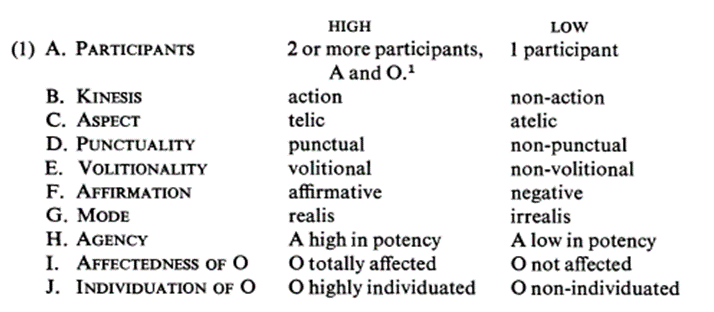
\includegraphics[width=12cm]{img/Hopper_transitivity.png}
    \caption{Elements constitutifs de la transitivité selon Hopper et Thompson (1980)}
    \label{Hopper_transitivity}
\end{figure}

Selon eux, plus une clause a de caractéristiques dans la colonne \textit{haut} (\textit{high}), plus elle est transitive. Ainsi, une phrase avec deux participants comme « Jerry aime la bière », où le patient \textit{bière} ne reçoit pas vraiment d'action, peut en réalité être moins bien notée qu'une phrase avec un seul participant, telle que « Susan est partie ».

Aussi, les auteurs notent que dans toutes les langues examinées au fil de leur étude (qui dépasse largement le cadre de l’anglais, l’approche étant précisément trans-culturelle), les éléments constitutifs de la transitivité covarient largement et systématiquement. Cela signifie qu'à chaque fois qu'une paire obligatoire de deux éléments de transitivité apparait dans la morphosyntaxe ou la sémantique d'une clause, les éléments appariés se trouvent toujours du même côté de l'échelle de la transitivité haute/basse. 

De là, ils considèrent la transitivité comme une propriété centrale de l'utilisation du langage. Probablement en raison d'une limitation psychologique dans le traitement du discours, elle servirait de signal morphosyntaxique des parties du discours qui doivent être stockées pour un traitement séquentiel immédiat (les parties dites « au premier plan » ou \textit{foregrounded}, qui communiquent la structure temporelle du récit), par opposition aux parties qui doivent être stockées pour une référence future ou un accès concomitant (les parties « en arrière-plan », ou \textit{backgrounded}, et qui ne contribuent pas immédiatement ni de manière cruciale à l'objectif du locuteur mais l'assistent, l'amplifient ou le commentent simplement). En bref, la probabilité qu'une clause reçoive une interprétation « de premier plan » est conçue comme proportionnelle à la hauteur de cette clause sur l'échelle de la transitivité. 

Sur la base de cet article, et en prenant le degré d’agentivité du participant comme caractéristique référentielle (ce que les auteurs appellent \textit{potency} ou \textit{agency}), on peut donc postuler que si un participant s’exprime, ou est exprimé, comme ayant plus d’agentivité, toute composante supplémentaire de transitivité présente dans la clause considérée devrait tendre corrélativement vers l'extrémité « haute » de l'échelle. Par exemple, si un événement est évoqué dans une phrase contenant un Agent au sens grammatical, composante linguistique qui semble ainsi la plus directement liée à la notion d’agentivité, cet événement aura tendance à être une action plutôt qu'un état. Et dans le cas particulier d’une action, cette dernière aura tendance à être (interprétée comme) plus volitive et/ou télique, c'est-à-dire représentée comme ayant une fin inhérente, naturelle ou volontaire. Enfin, si un objet est présent avec l'Agent dans une clause donnée, il aura tendance à être plus individué.

Une telle décomposition nous conduit à adopter une approche par faisceau d’indices, en tentant de construire un indice global d'agentivité intégrant toutes ces composantes, et qui devrait être globalement corrélé à l'agentivité du locuteur. L’idée ici est que même si certaines des composantes linguistiques incluses dans l’indice s'avèrent en réalité non corrélées, voire inversement corrélées avec l’agentivité par rapport à nos prédictions, l'indice devrait globalement évoluer dans la même direction que l’agentivité, tandis que des analyses successives pourront permettre de déterminer la qualité et la pertinence de chaque marqueur qui le compose.

Cela étant, la mesure du niveau d’agentivité d’un texte nécessite une modulation des indices proposés par Hopper et Thompson, l’agentivité n'étant plus simplement une composante parmi d'autres de la transitivité mais une variable dépendante à part entière. En ce sens, si l’on considère comme Hopper et Thompson que l'imposition de combinaisons linguistiques particulières dépend fondamentalement de la fonction dominante attribuée au langage, nous pourrions supposer qu’à la place du compromis entre \textit{foregrounding} et \textit{backgrounding} que les auteurs mettent en avant, ou bien au-delà de ce dernier, un compromis s’opère entre un usage purement « communicatif » de la langue et un usage « performatif » (au sens d’un langage conçu d’abord comme vecteur de construction identitaire par le locuteur-même), qui déterminerait l'utilisation préférentielle de constructions morphosyntaxiques potentiellement non chevauchantes, au-delà des seuls marqueurs lexicaux. Une telle conception fait directement écho à l'arbitrage théorisé par Vallacher\footnote{\cite{vallacher_levels_1989}} entre la bonne exécution d'une action (ici, raconter une histoire à quelqu’un) et la compréhension globale de ce qu'elle signifie pour soi (ici, faire du récit lui-même un enjeu identitaire, sujet récurrent en littérature et qui en ferait un champ d'étude privilégié, comme suggéré plus loin dans ce rapport).

Alternativement, si l'on considère que le langage sert toujours d’abord à communiquer, en retenant donc le fondement psychologique proposé par Hopper et Thompson, il est possible d'envisager qu’un langage plus agentif corresponde à un autre type de \textit{foregrounding} que celui mentionné par les auteurs, motivé par cette dimension psychologique spécifique qu’est l’agentivité. Plutôt que sa structure temporelle, le locuteur s’attacherait alors à mettre en avant la structure identitaire de son récit, ce qu'il dit sur son \textit{soi}. Là encore, ce \textit{foregrounding} pourrait impliquer des composantes linguistiques spécifiques, ne correspondant pas totalement à celles qui participent de la transitivité, ou efficacité temporelle, d’un discours. Néanmoins, l’on s’attendrait à trouver un certain nombre de convergences linguistiques entre ces deux motifs, l’agentivité étant crucialement dépendante de la capacité à adopter une perspective plus long-termiste, tel que le suggérait le modèle de Hitlin et Edler précédemment cité et les différentes manières de considérer le soi en fonction du cadre temporel adopté. Le soi peut en effet être considéré comme un instrument conceptuel nécessaire, un liant sémantique dont la fonction originelle serait précisément de permettre la pensée exploratoire\footnote{\cite{hills_foraging_2015}}, c'est-à-dire d'être orienté vers le futur, et ainsi de s’autoréguler à plus long terme par la rétrospection et l'anticipation, plutôt que de moduler sa performance dans le présent, focalisation caractéristique d’individus peu agentifs.

Si l’agentivité au sens grammatical (\textit{potency} ou \textit{agency}) du participant, sa volitionnalité et l’aspect télique de la clause en question, participant de sa transitivité selon Hopper et Thompson, peuvent également être considérés comme dénotant de manière concordante un degré supérieur d’agentivité, au sens de Vallacher, cela est cependant moins évident s'agissant de l'individuation de l'objet grammatical, définie par Hopper et Thompson de la manière suivante :

\begin{figure}[!ht]
    \centering
    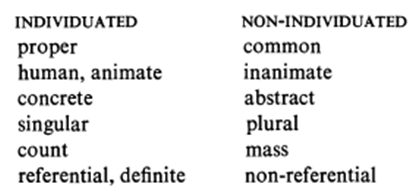
\includegraphics[width=8cm]{img/Hopper_individuation.png}
    \caption{Eléments participant de l'individuation de l'objet grammatical selon Hopper et Thompson (1980)}
    \label{Hopper_individuation}
\end{figure}

De fait, bien qu'elle soit considérée comme une composante transitive « faible » dans le tableau ci-dessus, nous nous attendons plutôt à ce que l'abstraction soit corrélée avec un niveau supérieur d’agentivité, étant donnée l’interprétation plus conceptuelle de leurs actions qui caractérise les agents « haut niveau ». Il en va de même pour les modes de l’irréel, classés par les auteurs dans la partie « basse » de l’échelle transitive. 

La direction de la corrélation, si elle existe, pour la composante d'affirmation n'est quant à elle pas évidente s’agissant d’agentivité. Cela peut s'expliquer par le fait qu’Hopper et Thompson définissent la transitivité comme l'\textit{efficacité} d'une action, à savoir son caractère plus ou moins réalisé, là où l’agentivité inclut également, pour reprendre la tripartition de Seligman\footnote{\cite{seligman_psychological_2023}}\footnote{\cite{seligman_psychological_2023}}, l'optimisme et l'imagination, que nous subsumerons sous la notion de « capacité de distanciation psychologique », ainsi que « l'auto-efficacité » ou « sentiment d’agentivité », qui n’est que partiellement corrélé à l’efficacité des actions entreprises par l’individu.

\section{Individualisme et pronoms : même méthode, nouveau raisonnement}

Le langage a souvent été utilisé comme un indicateur de dimensions psychologiques ou traits de personnalité spécifiques, ce à différents niveaux d'analyse. L'utilisation des pronoms en particulier, et leur lien avec la notion d'individualisme, a fait l'objet de nombreuses études. Nous précisons que toutes ces études traitent de l’anglais, et non du français. Néanmoins, et malgré l’existence de différences certes importantes entre ces deux langues, il semble n’y avoir aucune raison de penser qu'une approche psycholinguistique ne puisse s’appliquer au français également, et qu’elle révèlerait qui plus est les mêmes associations que celles décrites ci-après, étant donnés les marqueurs linguistiques relativement simples considérés ici, ainsi que les similitudes culturelles entre ces deux pays. 

Dans une étude de 1998, Kashima et Kashima\footnote{\cite{kashima_culture_1998}} ont constaté que l'augmentation de la richesse et le changement climatique prédisaient l'individualisme, mais que le résultat était modulé par l'utilisation de la langue : les cultures individualistes auraient tendance à favoriser l'utilisation explicite des pronoms de la première personne, tandis que les cultures collectivistes permettraient aux locuteurs d'abandonner les pronoms de la première personne dans la structure superficielle des phrases\footnote{Voir également \cite{yu_cultural_2016}}. De manière cohérente, l'utilisation de langues spécifiques, comme l'anglais, a été associée à des concepts de soi plus indépendants chez les personnes bilingues\footnote{\cite{marian_self-construal_2004}}. Plus généralement, des recherches antérieures ont établi un lien entre les pronoms de la première personne du singulier (tels que « je », « moi ») et l'individualisme d'une part, et entre les pronoms de la première personne du pluriel (tels que « nous ») et le collectivisme d'autre part\footnote{\cite{gardner_i_1999}}\footnote{\cite{kashima_culture_1998}}\footnote{\cite{na_culture_2009}}.  

Au sein d’une même culture, Twenge\footnote{\cite{twenge_changes_2013}} a pu observer que, dans les livres américains publiés entre 1960 et 2008, l'utilisation des pronoms de la première personne du pluriel avait diminué de 10\%, tandis que les pronoms de la première personne du singulier avaient augmenté de 42\%, et les pronoms de la deuxième personne (« tu », « toi ») quadruplé. Cela suggérerait d'après l'auteure la montée d'un individualisme aux Etats-Unis, avec une tendance parallèle vers moins de collectivisme.

Ces résultats peuvent être examinés à la lumière des recherches sur l'utilisation individuelle des pronoms : dans la correspondance personnelle et le discours, les pronoms singuliers de la première personne ont également été associés à une plus grande focalisation sur l'individu, ainsi qu'à un statut inférieur, à l'honnêteté, à la dépression et à un style plus personnel et plus expressif. A l’inverse, les personnes de statut supérieur utiliseraient davantage de pronoms de la première personne du pluriel et de la deuxième personne\footnote{\cite{nerbonne_secret_2014}}.

Si l’on tente de faire dialoguer ces deux niveaux d’analyse, culturel et individuel, les résultats de Twenge suggèrent donc que le langage (américain) aurait « évolué pour devenir moins hiérarchique, plus centré sur soi et plus expressif (peut-être dépressif) », bien que cela ne soit en accord qu'avec certains éléments de l'individualisme seulement (augmentation de l'expression émotionnelle, moins de hiérarchie dans l'ensemble, plus d'égocentrisme), mais pas nécessairement avec d'autres (plus d'excès de confiance et de revendication de statut, ce qui contraste avec l'association, au niveau individuel, entre un statut inférieur, l'honnêteté et la dépression d'une part, et l'utilisation de pronoms à la première personne du singulier d'autre part). L'utilisation de la deuxième personne en particulier, est associée à un statut supérieur et augmenterait avec le temps, de sorte que les résultats en matière de statut sont au mieux décrits comme mixtes.

Dans le même ordre d'idées, une analyse linguistique des 10 chansons américaines les plus populaires entre 1980 et 2007\footnote{\cite{dewall_tuning_2011}} a mis en évidence des changements dans l'utilisation de mots censés refléter des changements psychologiques : au fil du temps, l'utilisation de mots liés à la focalisation sur soi et au comportement antisocial aurait augmenté, tandis que les mots liés à la focalisation sur l'autre, aux interactions sociales et à l'émotion positive semblent avoir diminué.

Enfin, Twenge\footnote{\cite{twenge_generational_2012}} a constaté que, par rapport aux générations précédentes, un plus grand nombre d'étudiants américains se considèrent aujourd'hui comme « supérieurs à la moyenne » s'agissant d'attributs tels que les capacités académiques, la volonté de réussir, les capacités de leadership, la capacité à s'exprimer en public, la confiance en soi et la capacité à écrire (ce en tenant compte de la race, du sexe, des performances et du temps passé à étudier, ce dernier étant en fait en baisse ; et en dépit du fait que la population universitaire soit devenue moins sélective). L'auteure conclut que de vastes changements culturels mettant l'accent sur une vision positive de soi (aux États-Unis du moins) ont apparemment entraîné une amélioration des auto-évaluations dans les domaines agentifs, tandis que les auto-évaluations des attributs communautaires, tels que la compréhension des autres, la coopération et la spiritualité, auraient soit diminué, soit stagné. Aussi, les produits culturels, notamment dans leur forme linguistique, fonctionneraient à leur tour pour entretenir et accélérer de tels changements générationnels, vers la démonstration de traits psychologiques de plus en plus individualistes (en incluant dans cette notion aussi bien l'estime de soi, l’agentivité et le narcissisme).

Cependant, l'ambivalence du lien entre l'individualisme au niveau culturel et individuel mentionnée plus haut pose question, et pourrait laisser penser que l’agentivité est ici définie de manière trop restrictive. En effet, Twenge semble assimiler l’agentivité à un trait de personnalité parmi d'autres, qui résulterait de l'intériorisation d'un individualisme croissant au niveau culturel, les deux se renforçant alors mutuellement. En outre, cet individualisme est compris comme une valeur culturelle donnant la priorité à l'individu sur la collectivité, et est donc étroitement lié à l'affirmation de son propre statut dans le monde, vécu positivement. Non seulement ce raisonnement ne s'inscrit pas dans une approche évolutionnaire que nous expliciterons ci-après, mais nous adoptons une définition plus globale de l’agentivité personnelle, qui ne se résume pas à un jugement positif sur ses propres capacités individuelles, ou estime de soi. Twenge elle-même semble y faire allusion lorsqu'elle considère que ces auto-évaluations plus mélioratives des étudiants américains pourraient résulter, plutôt que d'un égocentrisme plus prononcé, du fait que «les étudiants récents interprètent les attributs de manière plus large que les générations précédentes, trouvant plus de façons de se considérer comme supérieurs à la moyenne »\footnote{\cite{dunning_ambiguity_1989}}. Cette « surinterprétation » correspondrait, en nos termes, à un niveau d’agentivité plus élevé, dans la mesure où un individu qui tend à identifier ses actions de manière plus abstraite au quotidien pourrait être corrélativement plus désireux et/ou capable d'extrapoler n'importe quelle notion, au-delà des actions seules, et d'en trouver ainsi une certaine définition selon laquelle on pourra dire qu'il est particulièrement performant - ce d’autant plus s’il s'agit de compétences métacognitives alors \textit{de facto} plus développées.

Si l'on peut s'attendre à ce qu'un niveau d'agentivité plus élevé favorise l'apparition de certains traits individualistes (narcissisme, extraversion, etc.), il n'y a donc pas de raison de postuler une correspondance biunivoque entre les deux concepts. La tendance au neuroticisme, par exemple, pourrait précisément être associée à un « débordement » de l'agentivité « haut niveau », ce contrairement à ce que l'individualisme appréhendé au niveau culturel semble prédire. Dans ce cas, l'individu serait incapable de passer à un niveau de conceptualisation engageant relativement moins son moi dans des situations nouvelles et/ou complexes, et serait donc amené à s’investir outre-mesure dans ce qui risque d'être mal exécuté, menaçant ainsi l'image de soi (comme le reflète le langage utilisé dans les communications personnelles).

Selon cette logique, il est alors possible de dépasser la conception péjorative de l'individualisme, définie comme un simple égocentrisme, pour le comprendre plutôt comme le corollaire naturel d'une plus grande agentivité, dont on rappelle l’orthogonalité supposée avec la communion.